\section{Experiments}

In this chapter, the three architectures described in the chapter \ref{Sec.SolutionDescription} are subject to different experiments. The architectures are evaluated using two metrics:
\begin{itemize}
\item Quality of future predictions evaluated by the expert.
\item Final score in an environment of the planning agent for different amounts of data collected.
\end{itemize}
The chapter starts with the OWM architecture, then move to the W+A architecture and finally arrive at the DPN architecture. Each approach was tested in Sokoban and Atari environments, except W+A which was tested only in the Boxing environment.

\subsection{OWM for Sokoban}

This section focuses on a problem of training OWM in Sokoban. The goal was to train the Memory module to generate sharp and accurate future predictions of observations and obtain high score of Controller playing in the environment.

\subsubsection{Train OWM in the Sokoban environment}

The Vision module successfully learned to encode high dimensional observations into low dimensional latent states. Fig.~\ref{Fig.WM_Sokoban_vision} shows original observations (first and third columns) side by side with reconstructed observations from their encodings (second and fourth columns). These are zero step predictions, no future is predicted only encoding to latent space and decoding to image space again is done.

\begin{figure}[H]
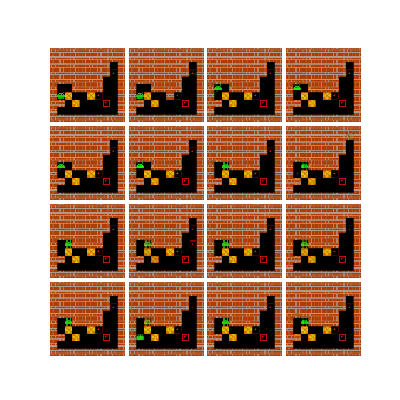
\includegraphics[width=0.7\textwidth,keepaspectratio]{figures/Sokoban_vision.png}
\caption[Qualitative result of the World Models' Vision module training in Sokoban]{Qualitative result of the Vision module training in Sokoban. First and third columns include original observations. Second and fourth columns include reconstructions. Each reconstruction was obtained by first encoding the original observation and then decoding it, using VAE encoder and decoder respectively.}
\label{Fig.WM_Sokoban_vision}
\end{figure}

It is hard to quantitatively measure the Memory module performance with e.g. log-likelihood. In practice, the single number does not tell much about quality of the predicted future states and its hard to interpret when the log-likelihood is high enough. In practice, though, it is far more useful to compare generated sequences of future observations with ground truth sequences with an eye of an expert, in this case the author of this thesis. What the expert looks for are sharp generated images which accurately resemble frames from the game. Moreover, the sequence needs to simulate subsequent actions properly, otherwise it is told that the sequence is noisy.

To generate a future prediction, 60 consecutive frames and actions from the dataset are fed into Memory to initialize its hidden state first. Then, when Memory is ready to generate future predictions, subsequent actions from the dataset and Memory own predicted latent states, as a contemporary states at following time steps, are fed into it to rollout the Memory module into the future. What gets generated are not frames, of course, but latent states. Those latent states are then decoded into images by Vision.

The stochastic and deterministic Memory modules were not able to learn Sokoban dynamics. Fig.~\ref{Fig.WM_Sokoban_memory} shows that the stochastic Memory module very often can not determine an agent position. The agent disappears and blocks change into other blocks. The eighth row shows that pushing mechanics are not modeled, the agent passes through boxes. The deterministic Memory module does not do better. \\
The Controller module failed to learn how to solve any level, it behaved comparably to a random play. We suspect that VAE is unable to generate high-level abstract Sokoban representation and the shallow Memory and Controller modules can not grasp complex dynamics of Sokoban using this poor representation. This idea is further developed in the next experiment.

\begin{figure}[H]
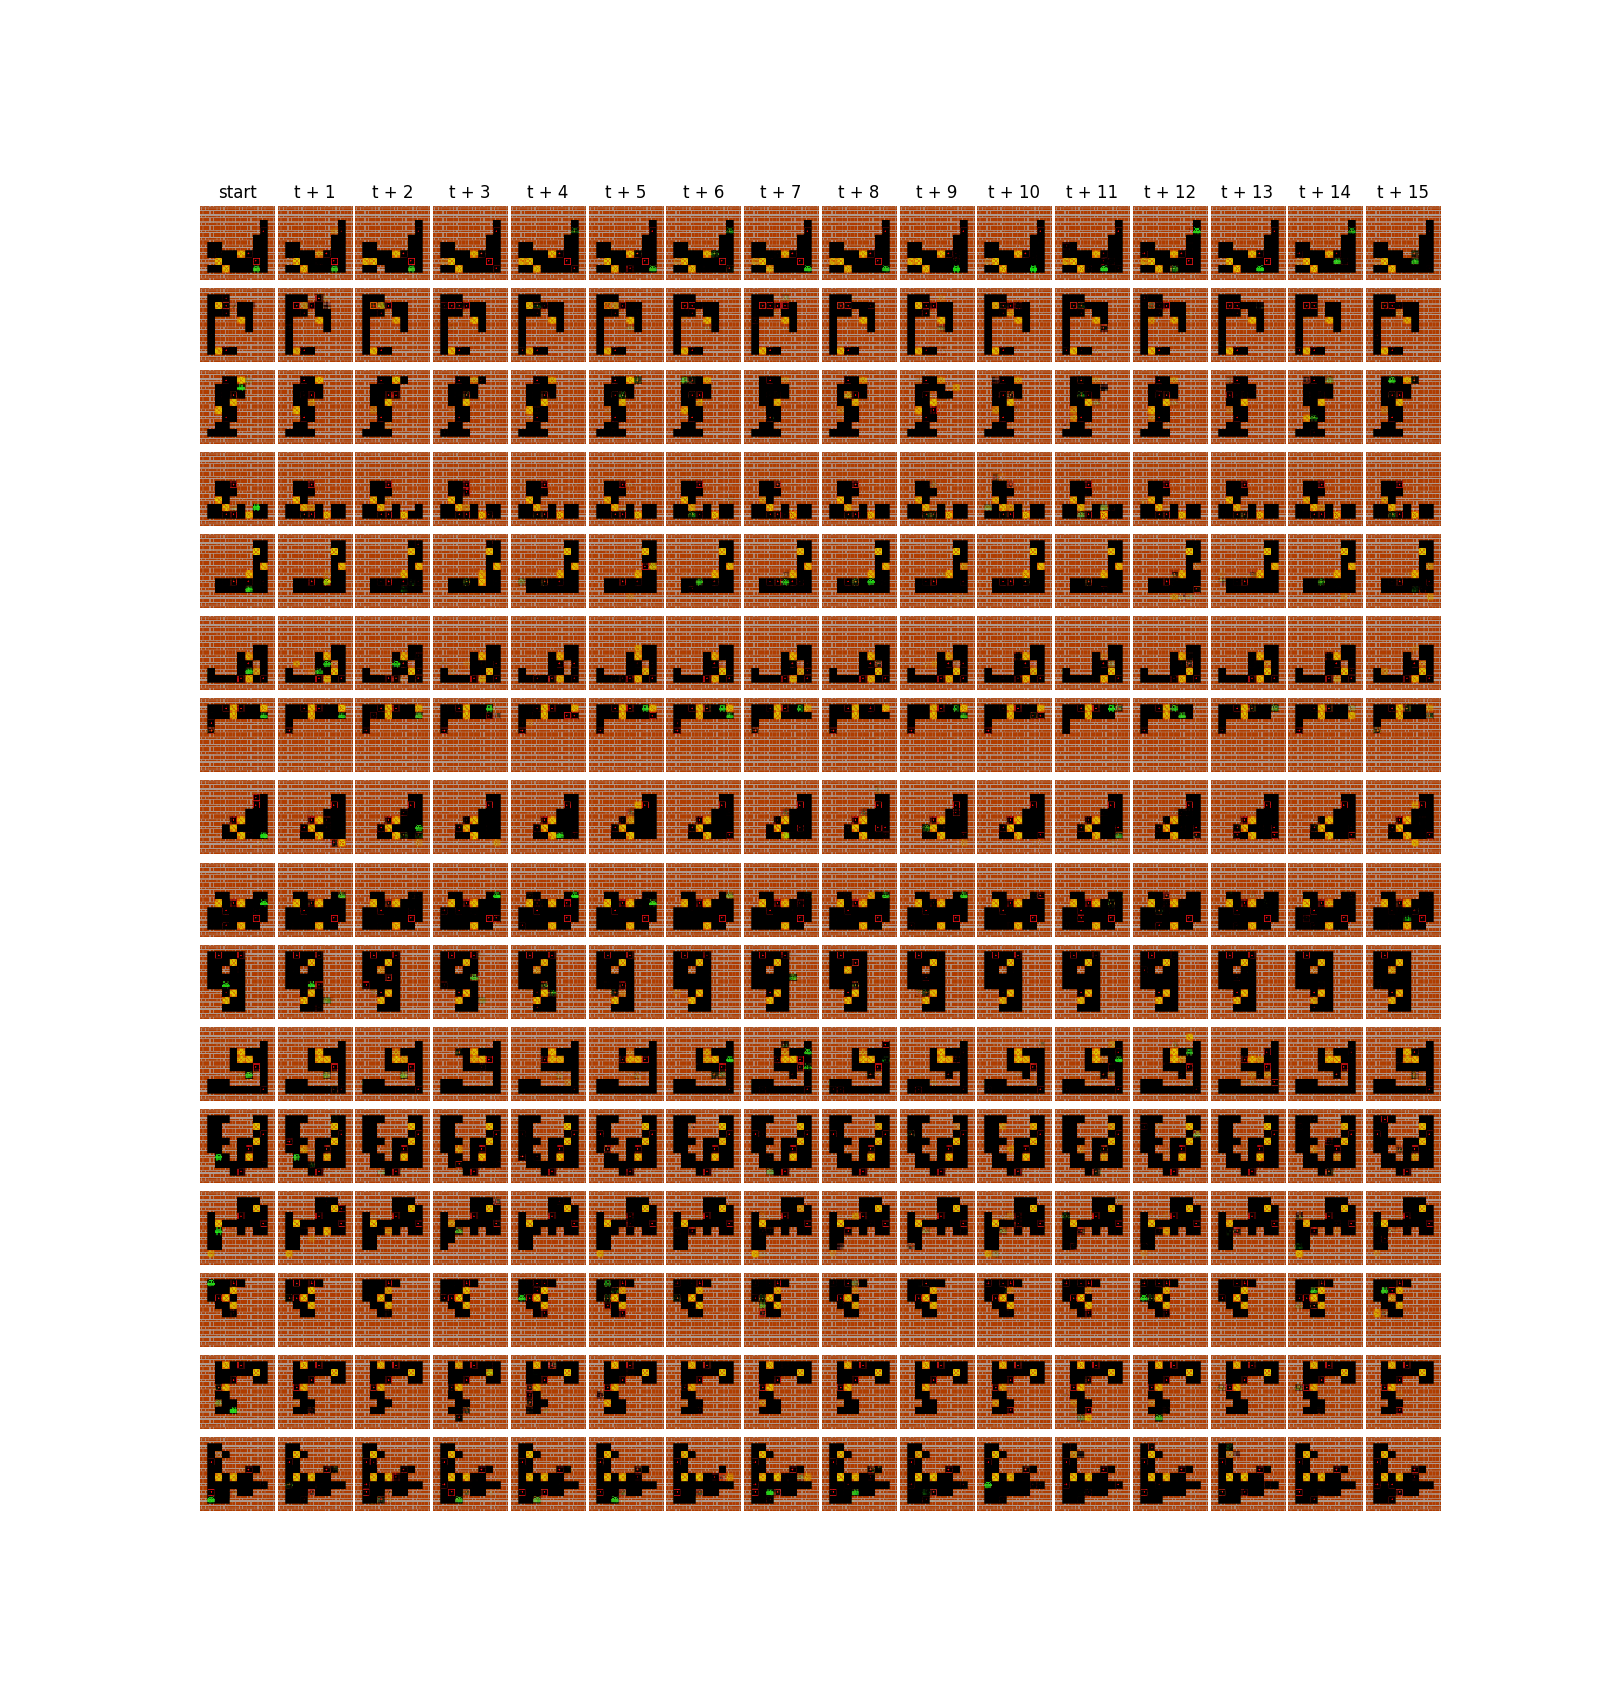
\includegraphics[width=1\textwidth,keepaspectratio]{figures/Sokoban_memory.png}
\caption[Qualitative result of the World Models' Memory module training in Sokoban]{Qualitative result of the Memory module training in Sokoban. Each column depicts the Memory module rollout in one episode. The first row include original observation from the evaluation dataset from which the rollouts start. The RNN's hidden state was initialized on preceding transitions in each episode. Each subsequent reconstruction was obtained by first predicting the next latent state by the Memory module and then decoding it using the VAE decoder.}
\label{Fig.WM_Sokoban_memory}
\end{figure}

\subsubsection{Train OWM in the Sokoban environment on 10x10 grid world states}

The latent state vector size is set to 64. This means that, in theory, this vector can accommodate full information about an observation. As noted before, Sokoban underlying game logic operates in a 10 × 10 grid world, where far edges of a level are always walls. This means that the level is described by 64 blocks organized in an 8 x 8 grid. In this experiment, this domain knowledge is exploited and the agent uses those 64 blocks as an input vector to the Memory module, bypassing the Vision module. It is worth noting, that the Vision module should learn this representation as it is the optimal encoding when the objective is to compress a pixel image into a 64-dimensional vector and then reconstruct the original observation from it. However, despite use of the optimal encoding, the results have not been improved.

The proposed input format is optimal encoding if one wants to compress a pixel image and then reconstruct it. However, it is really poor representation of a current state of the environment if one wants to use linear combination of those features (blocks in each position) to infer optimal next action and this is exactly what the Controller module is tying to do. Modeling a value function could have more sense e.g. the value function could learn that a box on a target position yields higher value, but even it would have a hard time modeling more complex relations between entities in the environment. More useful for the Controller would be e.g. representation that includes information about distance between the box and each target position. Nevertheless, this could be not enough too. The box on the target position would get discounted for not being on some other target positions. Hence, there is need for feature saying “the box X placed on the target position Y”. In the end, the linear combination of the proposed 64 raw features can not be used to learn good policy, better then a random play.

On the other hand, this representation includes, not well represented, but perfect information about an environment state. The Memory module creates its own environment representation encoded in its hidden state and then uses this representation to predict the next latent state. This Memory's hidden state is also utilized by the Controller. Still, it does not seem to encode useful enough information for the two, Memory and Controller, to do well on their tasks.

\subsubsection{Train OWM in the Sokoban environment with auxiliary tasks}

Auxiliary tasks \cite{Algo.AuxiliaryTasks} have proved to help create more informative representation of an environment. In this experiment, reward and value prediction tasks are added to the Memory module. In short, two additional linear models are added on top of the RNN to predict the next reward in the environment and model a value function. The reward head is trained in supervised manner to minimise MSE loss. The value head uses Monte-Carlo prediction algorithm, described in the section \ref{Sec.RL}, to estimate target states value and it is trained in supervised manner to minimise MSE loss just like the reward head. In theory, it should help form a more informative hidden state of the Memory module. Consequently, it should help learn Sokoban’s dynamics, but also generate representation on a higher level of abstraction that could prove useful for Controller. Moreover, the reward prediction will be needed in further work on planning with learned model.

For all that, the Memory module have not been able to learn to predict the rewards and values. Also, there was no improvement in Memory and Controller performance. It is suspected, that the main cause of this failure are sparse rewards in the training dataset. A random agent used to generate the dataset does not receive many positive rewards. Effectively, most of the episodes do not have any positive reward. Hence, the Memory module soon overfit on more or less constant reward and value. 
This yields insight that the data generation procedure does not cover state-space well. Iterative approach to gathering data, from a better and better agent, could solve this problem.

Moreover, it is not without significance that Sokoban has enormous state-space. Because each episode, or level, is randomly generated it is much different from the others - it is nearly impossible for an agent to see a similar state multiple times. Hence, Sokoban requires strong generalization capability from the Memory module. Simple RNN can lack capacity to create good representation and in turn achieve good prediction performance. A more flexible Memory module with larger capacity could manage this complexity and need for generalization.

The two insights from above are explored in the experiments with DPN, which have larger model and uses iterative training procedure.

\subsection{World Models for Atari}

Two more experiments below put World Models into the test. Firstly, OWN is trained in the Boxing environment, which has dense rewards and data collection using a random agent cover most of the state-space. If insights from the previous section are the only problems, then OWM should be able to achieve a good score in Boxing. \\
Then, the W+A architecture is tested in Boxing too.

\subsubsection{Train OWM in the Boxing environment}

The Vision module successfully learned to encode high dimensional observations into low dimensional latent states. Fig.~\ref{Fig.WM_Boxing_vision} shows original observations (first and third columns) side by side with reconstructed observations from their encodings (second and fourth columns). These are zero step predictions, no future is predicted only encoding to latent space and decoding to image space again is done.

\begin{figure}[H]
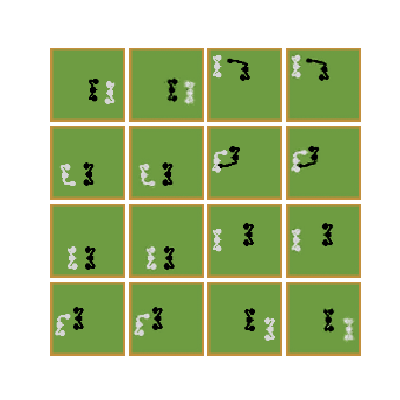
\includegraphics[width=0.7\textwidth,keepaspectratio]{figures/Boxing_vision.png}
\caption[Qualitative result of the World Models' Vision module training in Boxing]{Qualitative result of the Vision module training in Boxing. First and third columns include original observations. Second and fourth columns include reconstructions. Each reconstruction was obtained by first encoding the original observation and then decoding it, using VAE encoder and decoder respectively.}
\label{Fig.WM_Boxing_vision}
\end{figure}

The same procedure as in Sokoban was used to generate Memory observations predictions.

The stochastic Memory modules was able to learn Boxing’s dynamics. Fig.~\ref{Fig.WM_Boxing_memory} shows that the stochastic model generates very sharp and accurate predictions that model agents movement and punches really well. The agents does not disappear like in Sokoban and actions are smooth.
The Controller module successfully learned how to solve the game scoring above 18 points on average across 5 runs. OWM within its latent state of size 16 could be forced to encode two characters positions and hands states which are useful high-level features when deciding on the next action. It is worth pointing out here that similar experiment with such a small latent space did not yield improvement in Sokoban.

\begin{figure}[H]
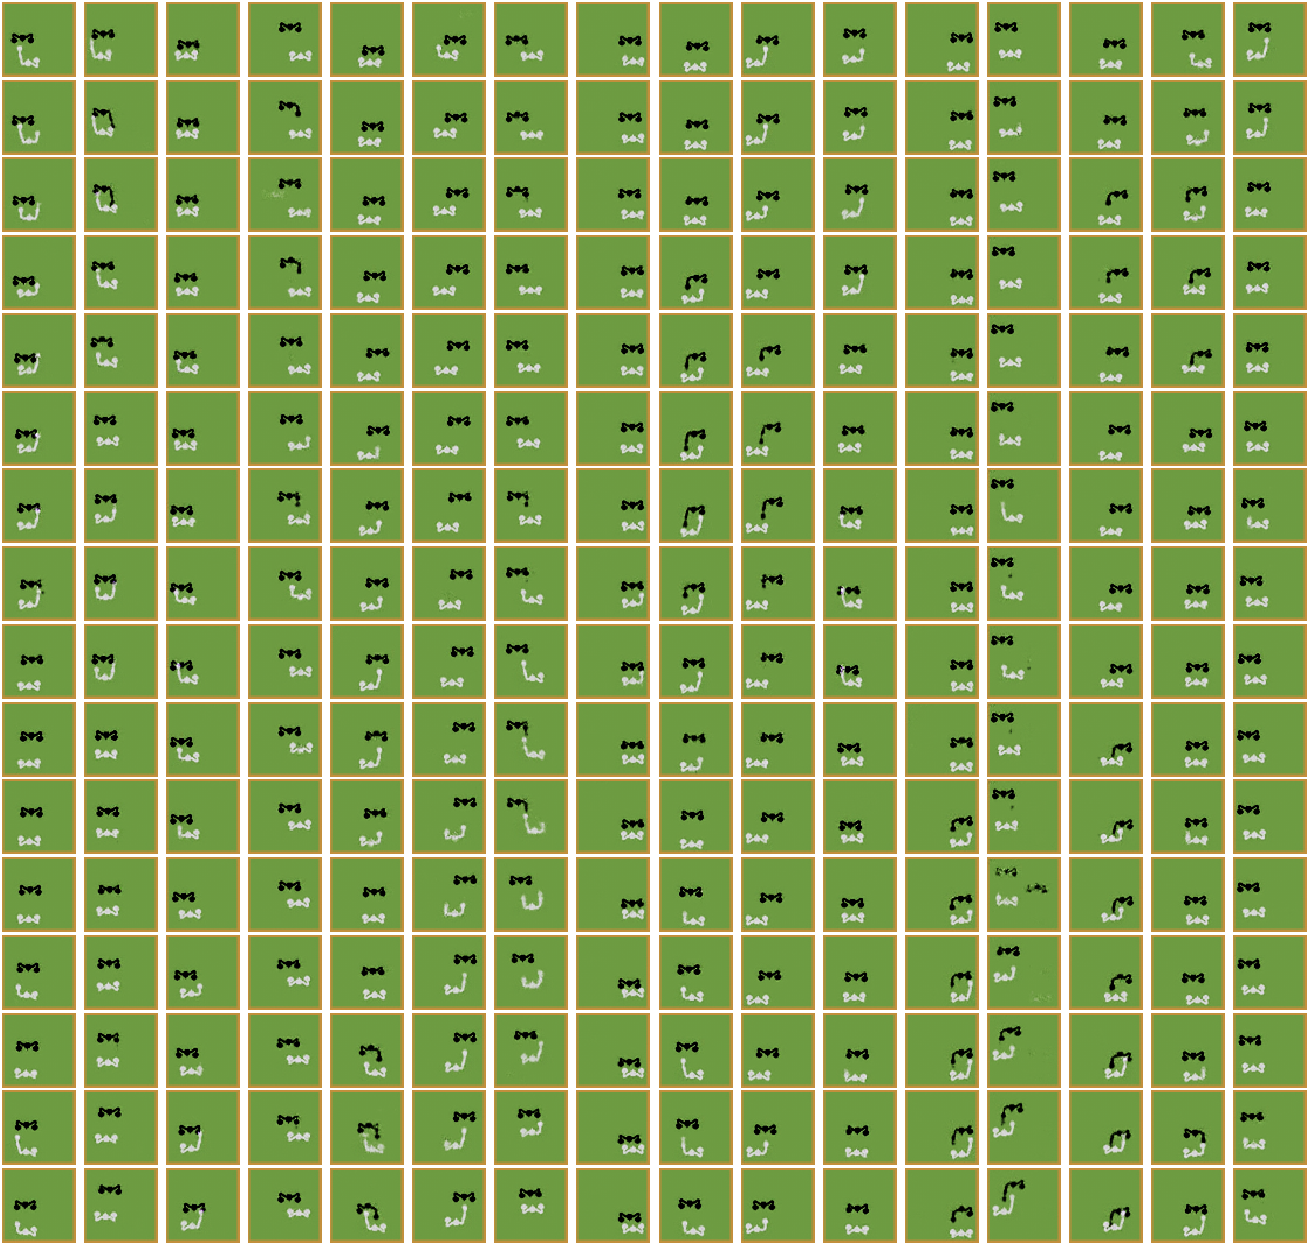
\includegraphics[width=1\textwidth,keepaspectratio]{figures/Boxing_memory.png}
\caption[Qualitative result of the World Models' stochastic Memory module training in Boxing]{Qualitative result of the stochastic Memory module training in Boxing. Each column depicts the Memory module rollout in one episode. The first row include original observation from the evaluation dataset from which the rollouts start. The RNN's hidden state was initialized on preceding transitions in each episode. Each subsequent reconstruction was obtained by first predicting the next latent state by the Memory module and then decoding it using the VAE decoder.}
\label{Fig.WM_Boxing_memory}
\end{figure}

\subsubsection{Train W+A in the Boxing environment}

Despite many attempts and hyper-parameter tuning, the deterministic Memory module was not able to model the Boxing dynamics as good as the stochastic one. This only proves that stochastic nodes are key for the accurate modeling. Fig.~\ref{Fig.WM_Boxing_deterministic_memory} shows future predictions which, as can be seen, are imperfect and noisy. The AlphaZero planner training was unstable and it did not train to properly plan using this model. Therefore, it was not able to play the game. Because the AlphaZero planner in its current form can only work with deterministic world models, decision was to abandon this solution and move to the DPN architecture.

\begin{figure}[H]
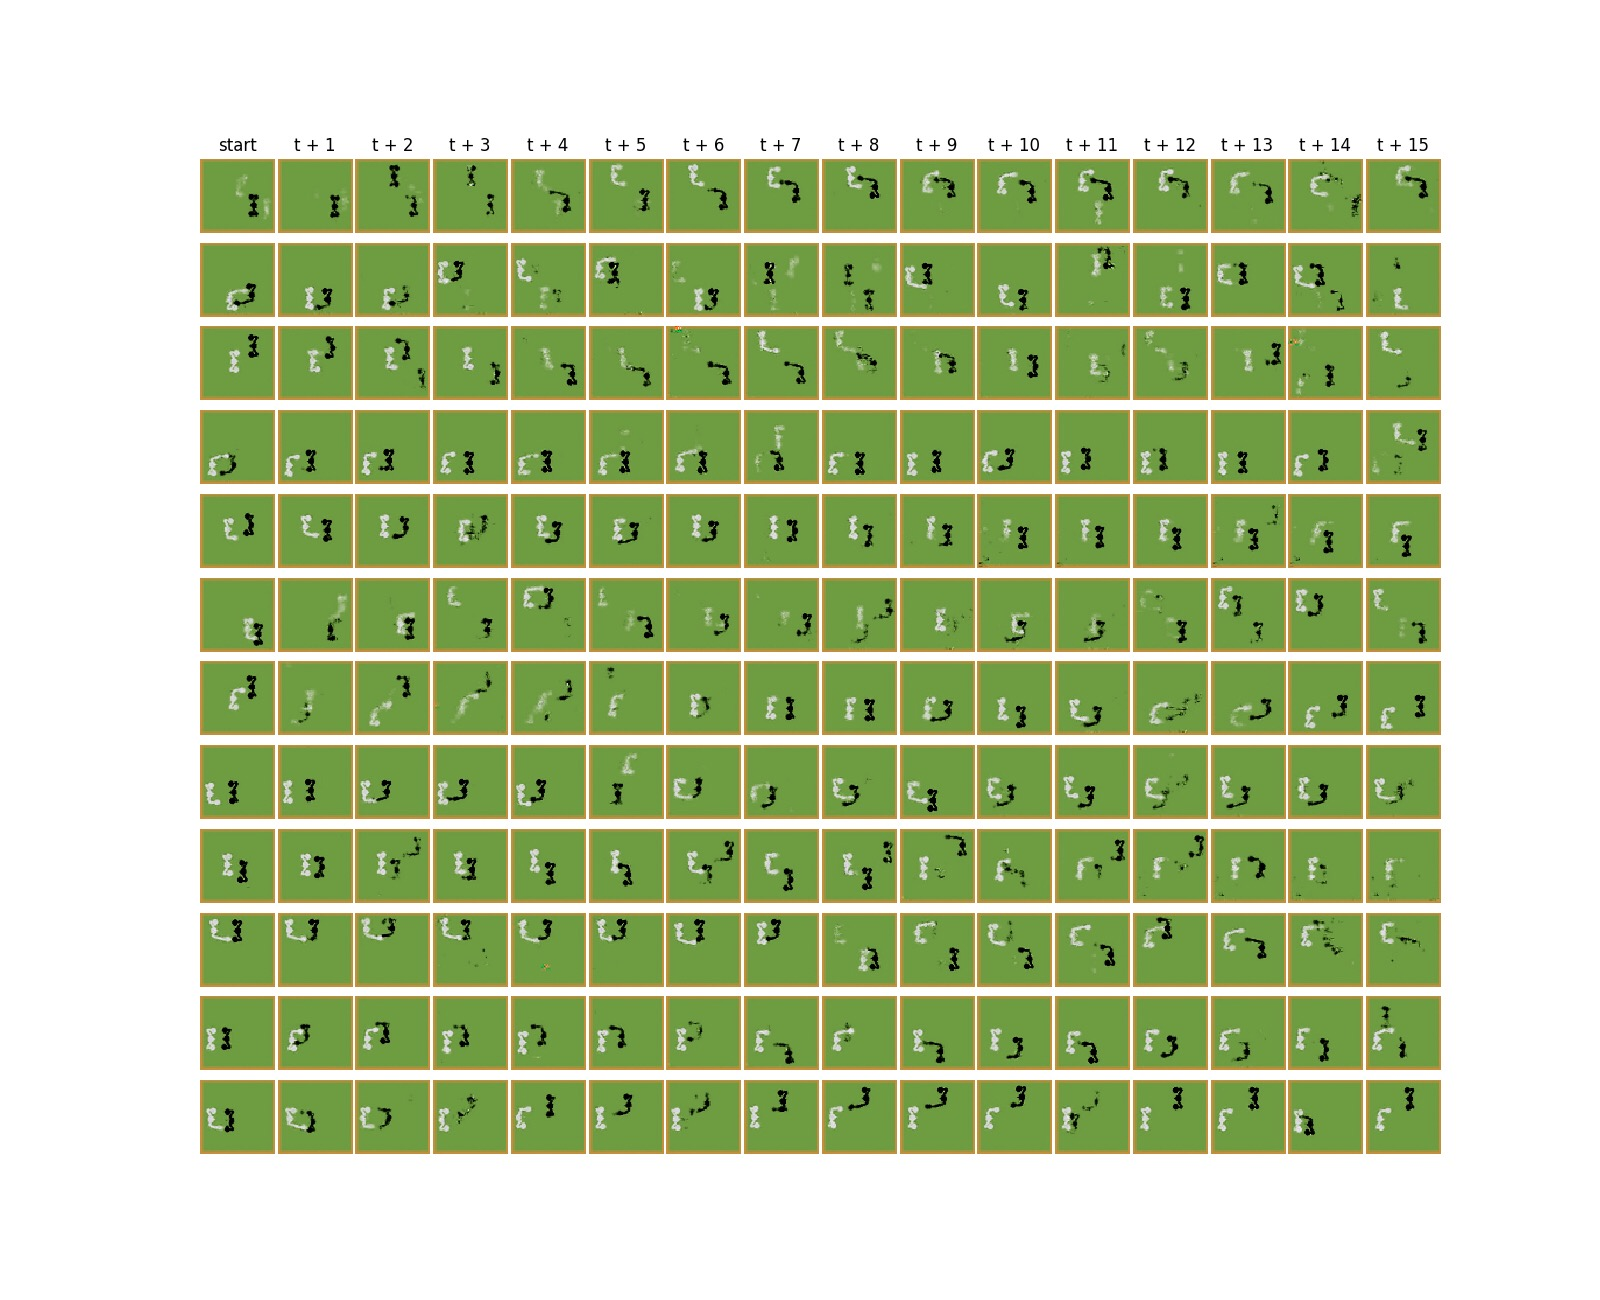
\includegraphics[width=1\textwidth,keepaspectratio]{figures/Boxing_deterministic_memory.JPG}
\caption[Qualitative result of the World Models' deterministic Memory module training in Boxing]{Qualitative result of the deterministic Memory module training in Boxing. Each column depicts the Memory module rollout in one episode. The first row include original observation from the evaluation dataset from which the rollouts start. The RNN's hidden state was initialized on preceding transitions in each episode. Each subsequent reconstruction was obtained by first predicting the next latent state by the Memory module and then decoding it using the VAE decoder.}
\label{Fig.WM_Boxing_deterministic_memory}
\end{figure}

\subsection{DPN for Sokoban}

\subsubsection{Train DPN in the Sokoban environment}

DPN could not capture Sokoban dynamics like OWM. In the figure below (Fig.~\ref{Fig.PlaNet_Sokoban_openloop}) future predictions are blurred, multiple agents appear and other artifacts, like changing blocks, are present. Similarly like in OWM case, the decision was to move to Atari games as easier environments to start with.

\begin{figure}[H]
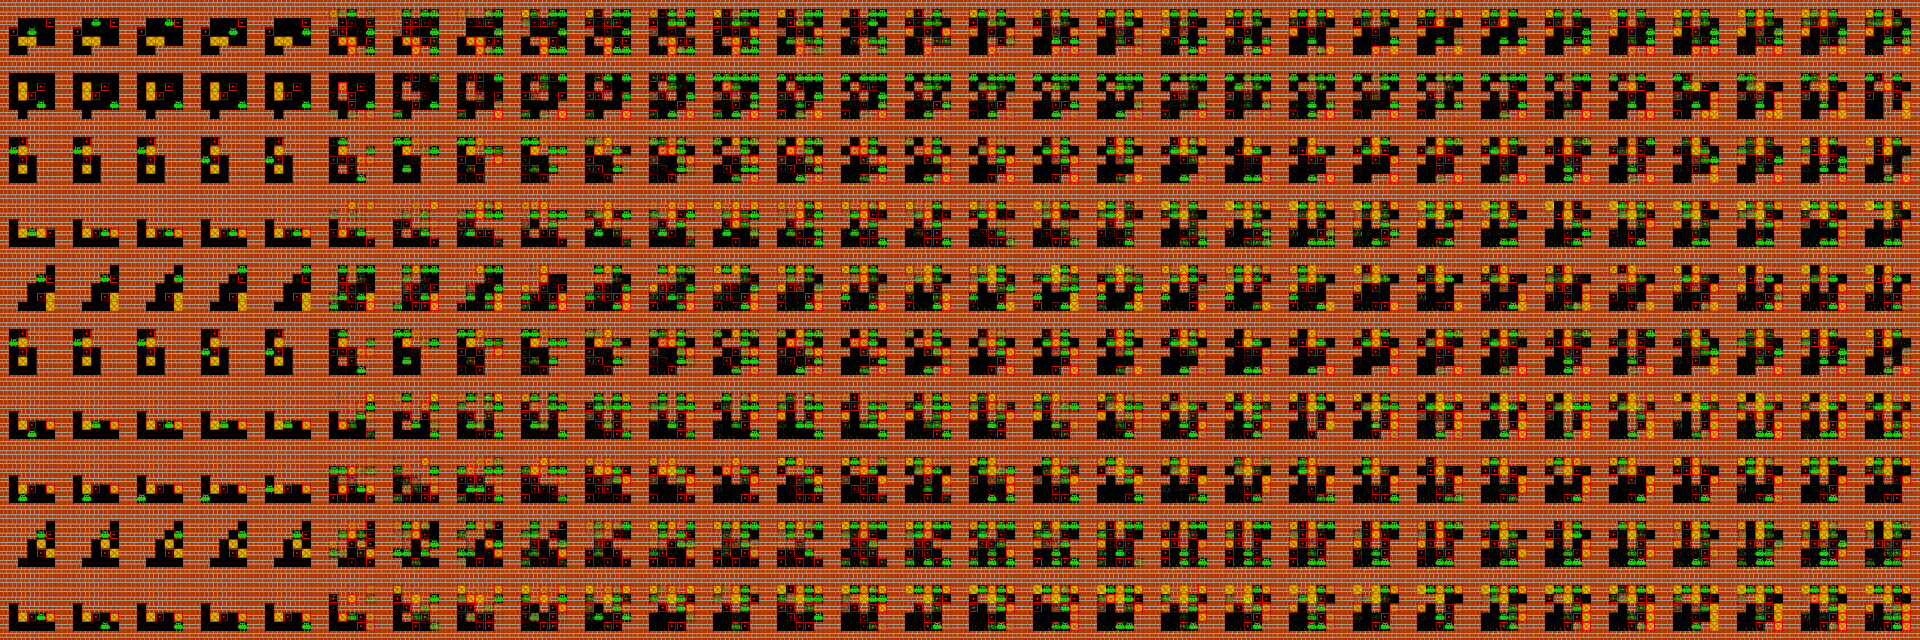
\includegraphics[width=0.9\textwidth,keepaspectratio]{figures/PlaNet/Sokoban_memory.png}
\caption[Qualitative result of the PlaNet model training in Sokoban]{Qualitative result of the model training in Sokoban. Each column depicts the model rollout in one episode. The first row include original observation from the evaluation dataset from which the rollouts start. Each subsequent reconstruction was obtained by first predicting the next latent state by the model and then decoding it using the decoder.}
\label{Fig.PlaNet_Sokoban_openloop}
\end{figure}

\subsection{DPN for Atari}

This section focuses on tuning DPN to yield high scores, comparable to model-free methods, preserving sample-efficiency of model-based methods.

\subsubsection{Train DPN in the Boxing environment}

DPN did not work out of the box with the default parameters from the original paper \cite{Algo.PlaNet}. Fig.~\ref{Fig.PlaNet_Boxing_original} shows that future predictions turn into a blurry blob, where it is not possible to distinguish one player from another.

By default a decoder variance of 1 is used, which means the model explains a lot of variation in the image as random noise. While this leads to more robust representations, it also leads to more blurry images. If the changes in consecutive frames are minor, then the posterior collapses because the model explains everything as observations noise. There are two possible solutions to this issue: one is to increase an action repeat and the other is to try to reduce the decoder variance. These are examined next.

\begin{figure}[H]
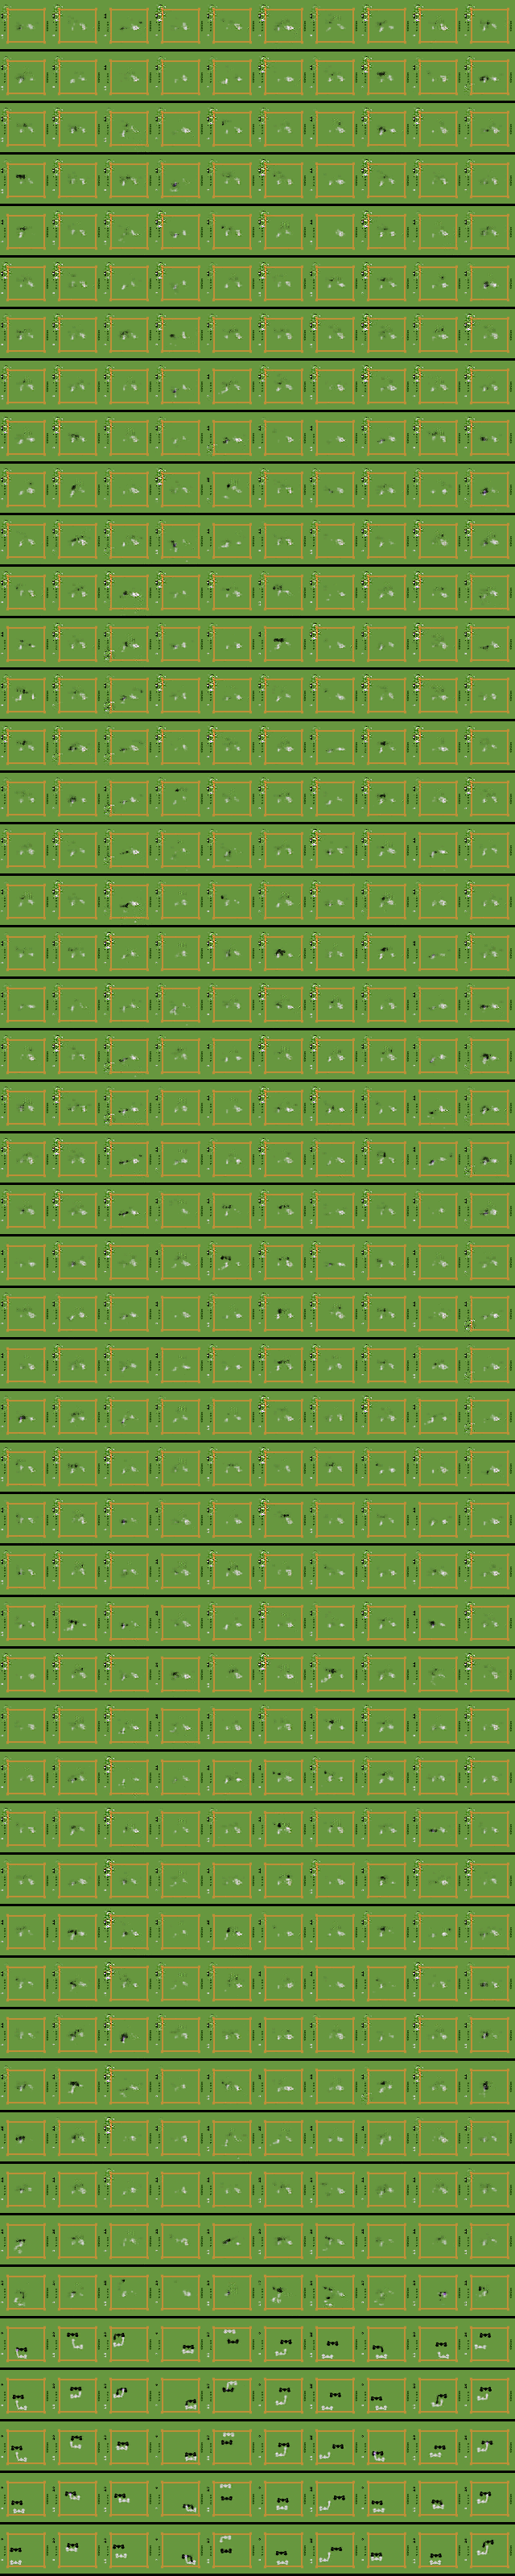
\includegraphics[height=0.9\textheight,keepaspectratio]{figures/PlaNet/Boxing_memory_original.png}
\caption[Qualitative result of the original PlaNet model training in Boxing]{Qualitative result of the model training in Boxing. Each column depicts the model rollout in one episode. The first row include original observation from the evaluation dataset from which the rollouts start. Each subsequent reconstruction was obtained by first predicting the next latent state by the model and then decoding it using the decoder.}
\label{Fig.PlaNet_Boxing_original}
\end{figure}

\subsubsection{Train DPN in the Boxing environment with the increased action repeat}

The action repeat will result in a bigger difference between consecutive frames and thus more signal for the model to learn from, that can not be easily modeled as noise. In practice though, it did not help and even made the agent play worse then a random agent.

\subsubsection{Train DPN in the Boxing environment with the lowered decoder variance}

The predictions are more blurry with a higher variance of a decoder because the decoder models more observations that differ slightly from the same latent code. This leads to the posterior, or the encoder, explaining more similar observations with the same code. If consecutive frames are very similar, then the posterior collapses and explain them with one code. By lowering the variance of the decoder it becomes more sensitive to small changes in observations and, hence, alleviate the problem of collapsing posterior when observations does not differ much from frame to frame.

To lower a decoder variance, the KL divergence scale is lowered, as explained in the section \ref{Sec.ModelLearning}. Other reason that lowering the divergence scale can help with collapsing posterior is that it allows the model to absorb more information from its observations by loosening the information bottleneck. On the other hand, it is recommended to keep the divergence scale as high as possible while still allowing for good performance. For instance, when the divergence scale is set to zero, it could learn to become a deterministic autoencoder which reconstruct observations well but is less likely to generalize to state in latent space that the decoder hasn't seen during training.

Random search resulted in the best divergence scale being around 0.03. It was tuned jointly with a free nats parameter which is described in the next section with detailed tuning results in the table \ref{Table.PlaNet_Boxing_tuning}.

\subsubsection{Train DPN in the Boxing environment with increased free nats}

The free nats technique, described in the section \ref{Sec.ModelLearning}, is used too. In case of Boxing, it helped to model boxers moves and actions more accurately. The best free nats turned out to be 12. Fig.~\ref{Fig.PlaNet_Boxing_lower_divergence_scale} shows final result.

\begin{figure}[H]
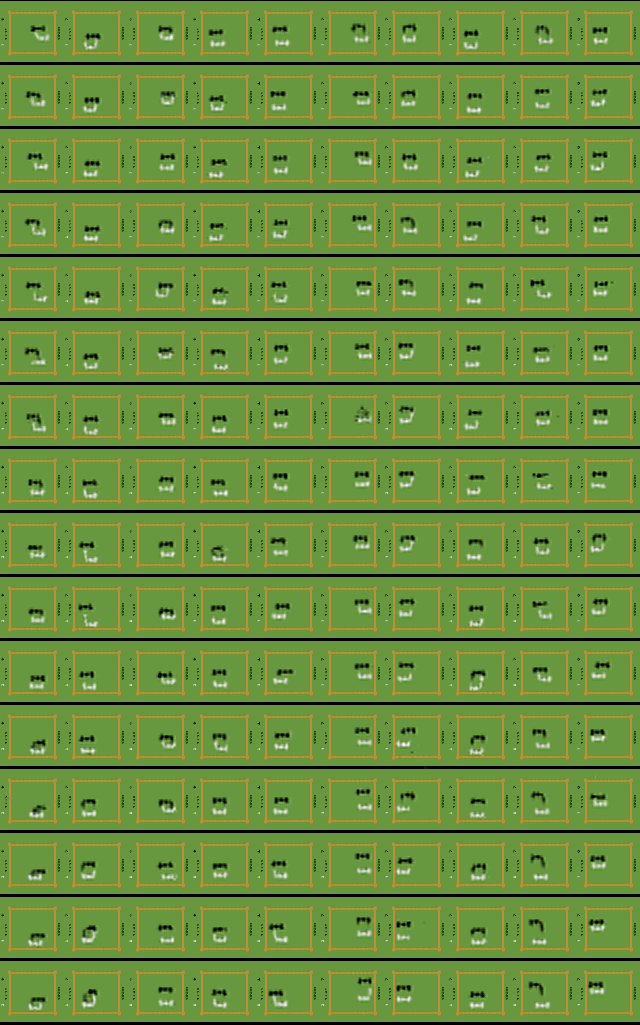
\includegraphics[height=0.9\textheight,keepaspectratio]{figures/PlaNet/Boxing_memory_sharp.png}
\caption[Qualitative result of the PlaNet model training with a lower divergence scale in Boxing]{Qualitative result of the model training in Boxing. Each column depicts the model rollout in one episode. The first row include original observation from the evaluation dataset from which the rollouts start. Each subsequent reconstruction was obtained by first predicting the next latent state by the model and then decoding it using the decoder.}
\label{Fig.PlaNet_Boxing_lower_divergence_scale}
\end{figure}

Table.~\ref{Table.PlaNet_Boxing_tuning} summarize hyper-parameters tuning experiment. The specialist evaluated noisiness of the model rollouts, the same as in fig.~\ref{Fig.PlaNet_Boxing_lower_divergence_scale}, in scale from 0 to 2, where 0 is a little or no noise in the future reconstructions and 2 is a lot of noise in the future reconstructions.

\begin{table}[H]
\centering
\begin{tabular}{| c | c | c |} 
\hline
Free nats & Divergence scale & Noisiness \\
\hline
2  & 1E-04 & 2 \\
16 & 1E-04 & 2 \\
13 & 1E-04 & 2 \\
11 & 2E-04 & 2 \\
3  & 2E-04 & 2 \\
1  & 3E-04 & 2 \\
8  & 3E-04 & 2 \\
4  & 4E-04 & 2 \\
17 & 1E-03 & 2 \\
7  & 2E-03 & 2 \\
10 & 2E-03 & 2 \\
15 & 2E-03 & 2 \\
6  & 2E-03 & 2 \\
9  & 3E-03 & 2 \\
13 & 4E-03 & 2 \\
15 & 4E-03 & 2 \\
15 & 5E-03 & 2 \\
8  & 5E-03 & 2 \\
5  & 6E-03 & 2 \\
10 & 1E-02 & 1 \\
4  & 2E-02 & 1 \\
8  & 2E-02 & 0 \\
17 & 3E-02 & 0 \\
12 & 1E-01 & 0 \\
\hline
\end{tabular}
\caption{PlaNet for Boxing hyper-parameters tuning results.}
\label{Table.PlaNet_Boxing_tuning}
\end{table}

The lower divergence scale the nosier predictions are. The higher free nats the better, more stable, movement predictions are. Best params turned out to be: the divergence scale around 3E-02 and the free nats around 12.

It achieved final score around 45 after 1 million steps of data collection in the environment. The learning curve is shown in fig.~\ref{Fig.Boxing_with_overshooting}.

\begin{figure}[H]
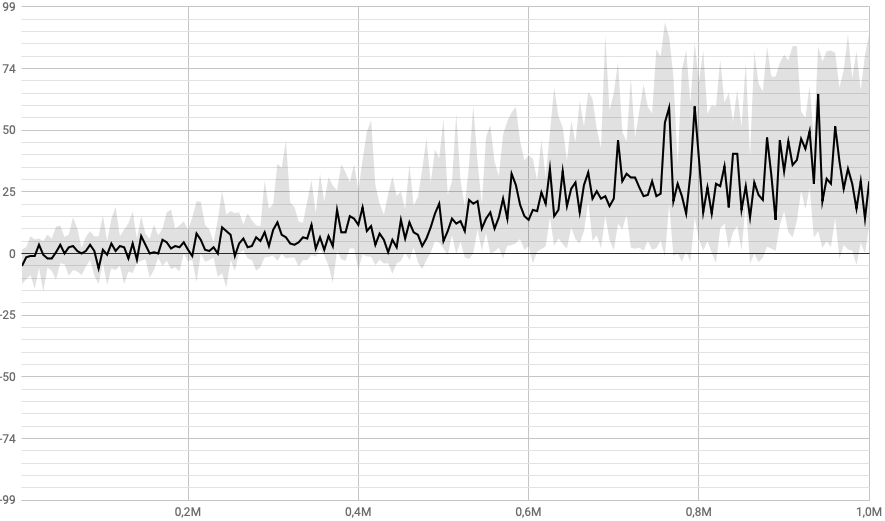
\includegraphics[width=0.8\textwidth,keepaspectratio]{figures/PlaNet/Boxing_with_overshooting.png}
\caption[Boxing learning curve after tuning and with overshooting]{Boxing learning curve after tuning and with overshooting. The line presents median and the shaded area are percentiles 5 to 95 over 5 training runs. On the Y axis is the environment score and on the X axis is number of steps in the real environment for the data collection.}
\label{Fig.Boxing_with_overshooting}
\end{figure}

\subsubsection{Train DPN in the Freeway environment}

The same random search procedure was applied to the Freeway environment described earlier. Fig.~\ref{Fig.PlaNet_Freeway_lower_divergence_scale} shows final result.

\begin{figure}[H]
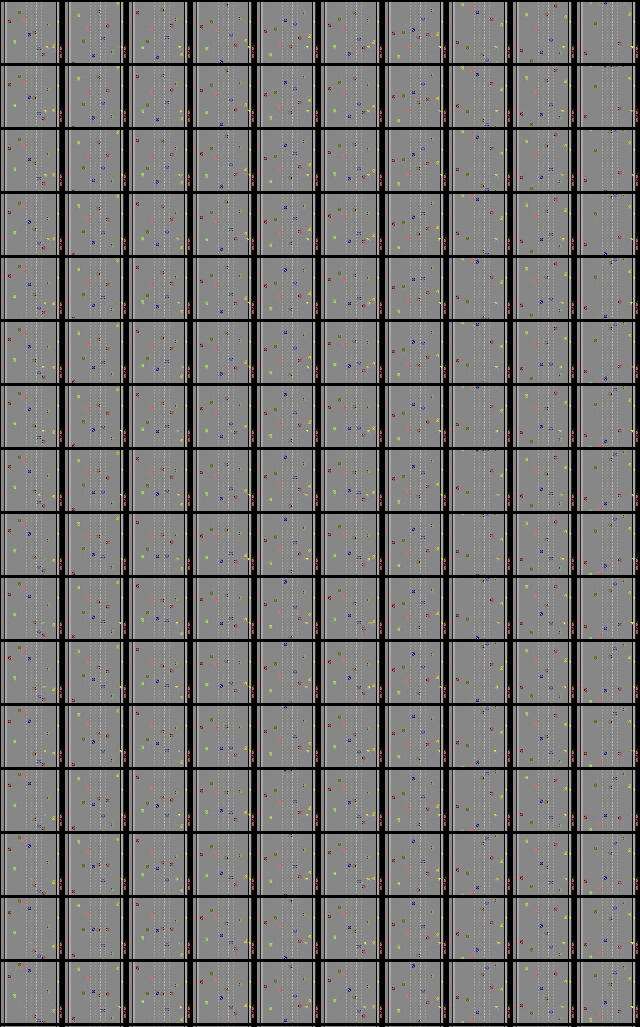
\includegraphics[height=0.9\textheight,keepaspectratio]{figures/PlaNet/Freeway_memory_sharp.png}
\caption[Qualitative result of the PlaNet model training with a lower divergence scale in Freeway]{Qualitative result of the model training in Freeway. Each column depicts the model rollout in one episode. The first row include original observation from the evaluation dataset from which the rollouts start. Each subsequent reconstruction was obtained by first predicting the next latent state by the model and then decoding it using the decoder.}
\label{Fig.PlaNet_Freeway_lower_divergence_scale}
\end{figure}

Table.~\ref{Table.PlaNet_Freeway_tuning} summarize hyper-parameters tuning experiment conducted in the same way like for Boxing.

\begin{table}[H]
\centering
\begin{tabular}{| c | c | c |} 
\hline
Free nats & Divergence scale & Noisiness \\
\hline
9 & 8E-02 & 2 \\
6 & 2E-02 & 2 \\
5 & 3E-03 & 2 \\
4 & 6E-04 & 2 \\
4 & 4E-04 & 2 \\
4 & 2E-04 & 2 \\
7 & 3E-02 & 1 \\
6 & 5E-04 & 1 \\
4 & 1E-04 & 1 \\
2 & 2E-04 & 1 \\
5 & 8E-03 & 0 \\
2 & 2E-03 & 0 \\
\hline
\end{tabular}
\caption{PlaNet for Freeway hyper-parameters tuning results.}
\label{Table.PlaNet_Freeway_tuning}
\end{table}

High free nats, above 6, and too low, below 1E-03, or too high, above 9E-03, divergence scale makes future predictions very noisy and blurry. Best parameters chosen were: the divergence scale of 8E-03 and the free nats of 3.

Despite really good future observations prediction, the agent failed to reliably play the game with high score. Results in fig.~\ref{Fig.Freeway_with_overshooting} show that the agent in the early phase of the training, when the model is still untrained and returns mostly random signals, does better then in the late training phase, when the model predicts next states and rewards well. One explanation of this phenomena is that a planner horizon is too short to cover a plan which ends with a positive reward on the other side of the road. The longer planning horizon might help and this is explored in the next experiment.

\begin{figure}[H]
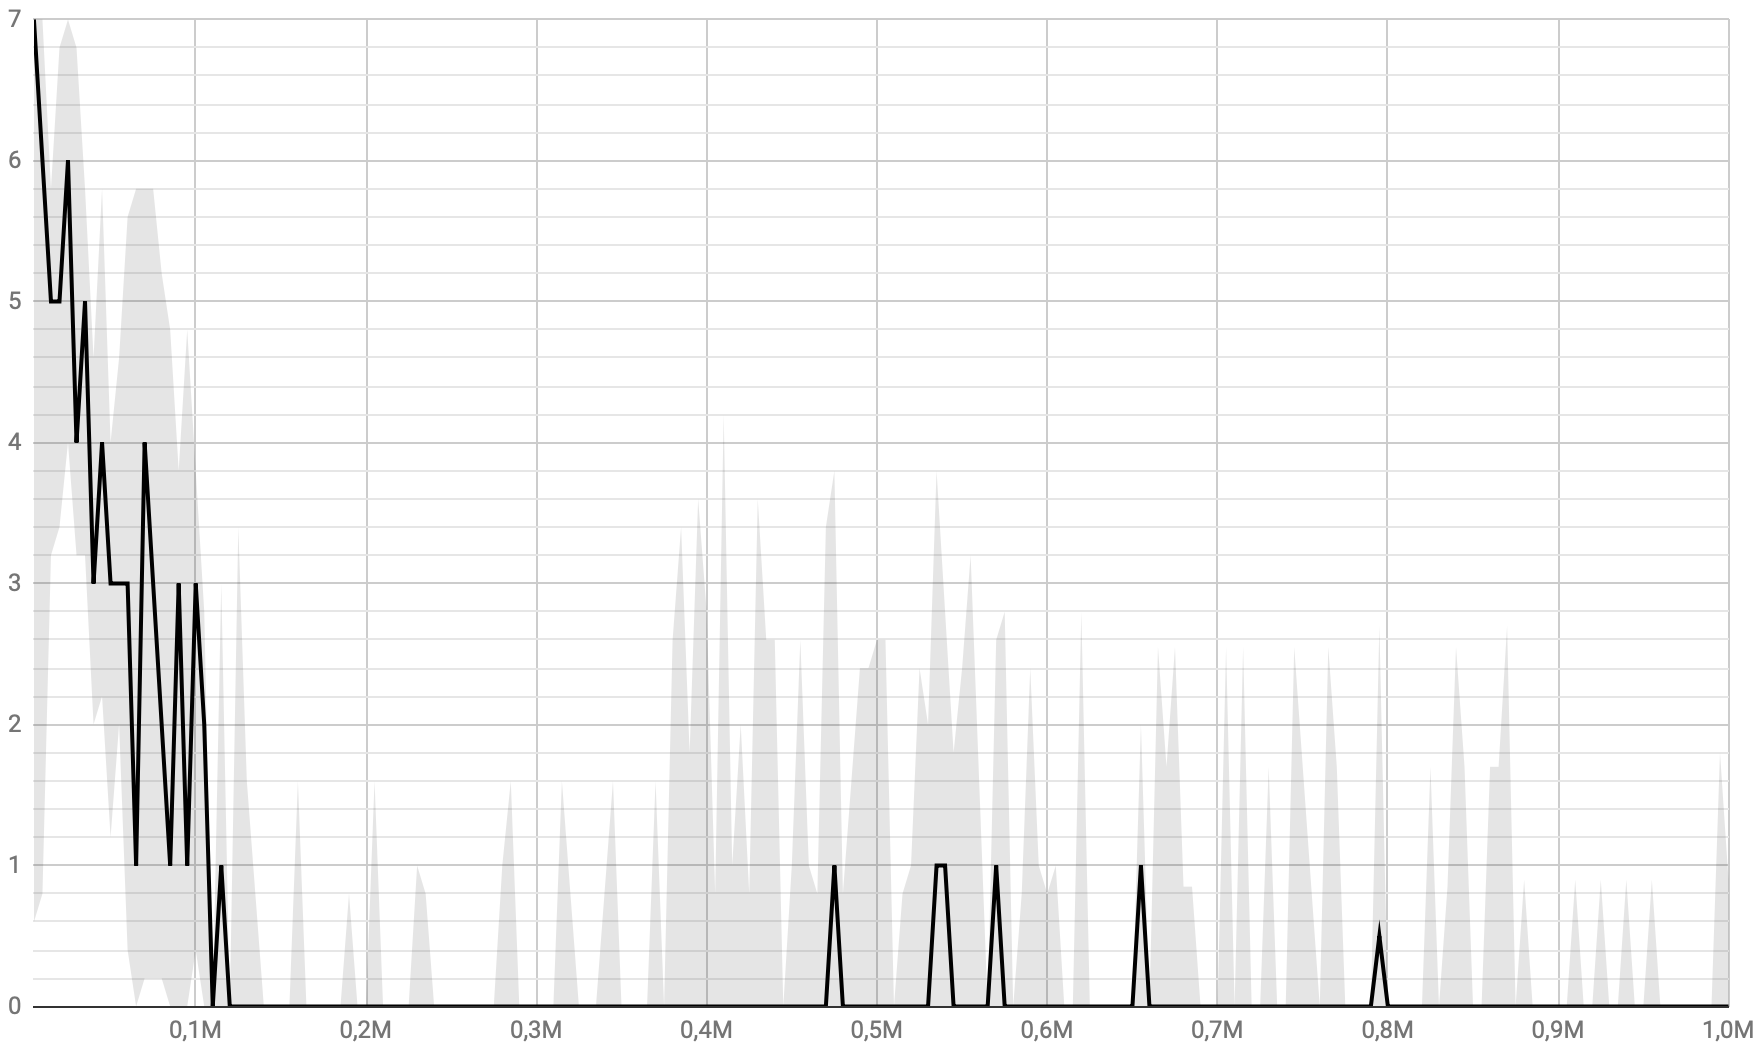
\includegraphics[width=0.8\textwidth,keepaspectratio]{figures/PlaNet/Freeway_with_overshooting.png}
\caption[Freeway learning curve after tuning and with overshooting]{Freeway learning curve after tuning and with overshooting. The line presents median and the shaded area are percentiles 5 to 95 over 5 training runs. On the Y axis is the environment score and on the X axis is number of steps in the real environment for the data collection.}
\label{Fig.Freeway_with_overshooting}
\end{figure}

\subsubsection{Train DPN in the Freeway environment with a longer planning horizon}

Two experiments were run: first for planning horizon of 25 and second for planning horizon of 50. Both failed to improve the agent score. After many attempts, the Freeway environment was left unsolved.

\subsubsection{Train DPN in the Boxing environment without overshooting}

The authors in the final version of the original PlaNet paper \cite{Algo.PlaNet} found out, that disabling overshooting can increase performance for their RSSM architecture. It was put into the test and final results are shown in fig.~\ref{Fig.Boxing_without_overshooting}. It helped increase performance of DPN tuned for Boxing.

\begin{figure}[H]
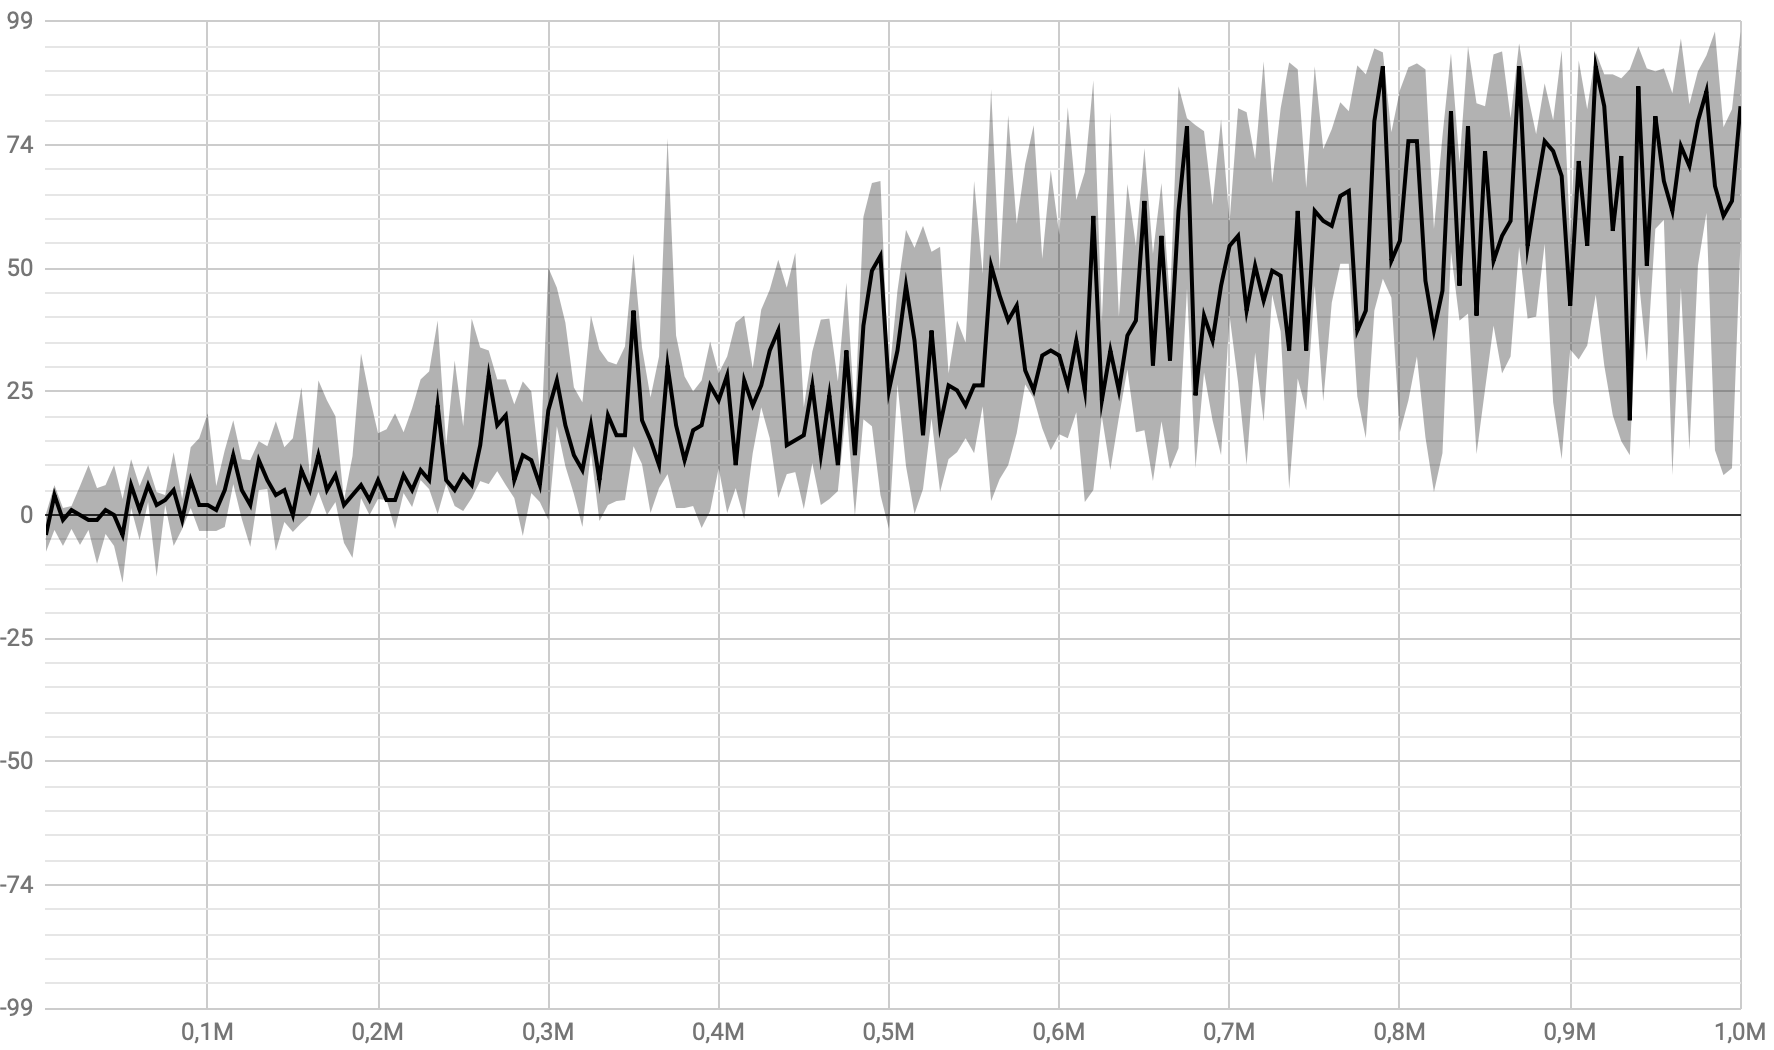
\includegraphics[width=0.8\textwidth,keepaspectratio]{figures/PlaNet/Boxing_without_overshooting.png}
\caption[Boxing learning curve after tuning and without overshooting]{Boxing learning curve after tuning and without overshooting. The line presents median and the shaded area are percentiles 5 to 95 over 5 training runs. On the Y axis is the environment score and on the X axis is number of steps in the real environment for the data collection.}
\label{Fig.Boxing_without_overshooting}
\end{figure}

This is the best and final solution which gets compared to strong model-based baseline SimPLe \cite{Algo.SimPLe} and model-free baselines Rainbow \cite{Algo.Rainbow} and PPO \cite{Algo.PPO}. Score of randomly issuing actions in the environment is also reported. Comparison is done in low data regime of 100K, 500K and 1M interactions with the real environment. The baseline results are taken from the SimPLe paper \cite{Algo.SimPLe}.

\begin{table}[H]
\centering
\begin{tabular}{|c | c c c|} 
\hline
Algo.   & 100K        & 500K        & 1M          \\
\hline
Ours    &  6,2 (10,7) & 35,2  (8,3) & 78,2 (19,1) \\ 
SimPLe  &  9,1  (8,8) & NDA         & NDA         \\
PPO     & -3,9  (6,4) &  3,5  (3,5) & 19,6 (20,9) \\
Rainbow &  0,9  (1,7) & 58,2 (16,5) & 80,3  (5,6) \\
Random  & \multicolumn{3}{c|}{0,3}                \\
\hline
\end{tabular}
\caption[Results comparison]{Mean scores and standard deviations (in brackets) over five training runs.}
\label{Table.Results}
\end{table}

Tuned DPN architecture without overshooting is better than PPO in every data setting and from Rainbow in low data regime of 100K interactions with the real environment. The performance is also comparable with SimPLe in all data settings and with Rainbow in 500K and 1M data settings. Therefore, it is clear that the DPN architecture is sample-efficient without sacrificing final performance of the agent.
